%% Placement Is Provenance — IEEE journal manuscript
%%
%% Build:  tectonic main.tex
%%
%% Every number in this file is traceable to docs/paper/*.md, which record the
%% run that produced it. Where a claim would flatter the method beyond what the
%% data supports, the weaker claim is made instead; Section IX states results
%% that argue against our own approach.
\documentclass[journal]{IEEEtran}

\usepackage{cite}
\usepackage{amsmath,amssymb}
\usepackage{graphicx}
\usepackage{booktabs}
\usepackage{url}
\usepackage[hidelinks]{hyperref}

\begin{document}

% The title scopes the claim. The method is a join over parser output with
% nothing language- or genre-specific in it, and the headline result is on an
% external English benchmark, so the title must not name the deployment.
\title{Placement Is Provenance: Anchor-Preserving Ingestion for\\
Figure-Grounded Retrieval-Augmented Generation}

% TODO(camera-ready): the author list is deliberately unfilled. Replace both
% blocks below, and the matching fields in ../CITATION.cff.
\author{\IEEEauthorblockN{Author list withheld pending submission}%
\thanks{Manuscript prepared 13 August 2026. Corresponding author: \texttt{author@example.org}.}}

% TODO(camera-ready): venue. This header names a learning-technologies journal,
% which fits the deployment but not the claim; a multimedia / data-engineering
% venue matches the contribution better.
\markboth{Preprint (draft)}%
{Placement Is Provenance: Anchor-Preserving Ingestion for Figure-Grounded RAG}

\maketitle

\begin{abstract}
Multimodal retrieval-augmented generation is evaluated almost entirely on
\emph{which} evidence is retrieved. A tutoring system that shows figures from a
textbook is judged on a second axis as well: \emph{where} the figure lands in the
explanation. We show that this axis is separable, that it is cheap to measure, and
that the information determining it is produced by every layout parser and
routinely discarded before serving.

The method is a join over data the parser already produced, not a model: it is
independent of language and of document genre. We evaluate it on both. On
MRAMG-Bench's Academic subset --- English arXiv documents whose gold image lists
were written by ten graduate-student annotators in computer science, each
assigned papers in their own field --- a 568M-parameter cross-encoder over anchor-derived context
reaches Image Precision \textbf{69.63}, and \textbf{67.50} under forced emission,
against 65.28 for the best published system (GPT-4o). The configuration was frozen
before that dataset was obtained.

For development and stress testing we release a caption-scarce stress corpus of
Indonesian K--12 curriculum textbooks: 13 government titles,
2{,}816 pages, extracted through two independent pipelines, with 486 adversarially
filtered questions. This corpus is not the scope of the claim but its hardest
case: only a fifth of its figures carry a printed caption, so the failure this
paper is about is visible there and largely hidden in caption-rich corpora. We
introduce a \emph{layout-gold placement metric} that derives placement ground
truth from the source document's own typesetting at no per-item annotation cost,
and a headline \emph{Grounded Figure F1} that credits a figure only when it is
both the right figure and in the right place.

Two findings require no model and replicate across both extraction pipelines. Only
19.3\,\%/34.3\,\% of figures carry a printed caption, while \textbf{100\,\%} carry
a recoverable reading-order anchor. And under perfect retrieval \emph{and} a
perfect answer, caption-based placement is still off by 2.08/4.69 sentences.
Placement is not implied by retrieval. Notably, the corpus with nearly twice the
caption coverage places \emph{worse}, because its share of lexically
indistinguishable figures also doubles: caption availability is not caption
discriminability.

On the textbook corpus, composing a vision-language filter with that same
cross-encoder raises figure-selection precision from 0.028 to \textbf{0.542}
against human annotation --- sight for recall, discrimination for precision.

\end{abstract}

\begin{IEEEkeywords}
Multimodal retrieval-augmented generation, document layout analysis, figure
grounding, document ingestion, cross-encoder reranking.
\end{IEEEkeywords}

\section{Introduction}

\IEEEPARstart{A}{n} AI study assistant grounded in school textbooks must do more
than quote the right paragraph. Curriculum books teach substantially through
pictures: a labelled water-cycle diagram, a food-chain chart, a worked geometric
construction. When such a system answers a child's question, showing the right
figure at the right point in the explanation is part of the answer, not decoration
around it.

Two distinct things can go wrong. The system can show the \textbf{wrong figure}, or
it can show the \textbf{right figure in the wrong place} --- after the explanation
has moved on, or bundled at the end where the reader must reconstruct which
sentence it belongs to. The first failure is measured everywhere. The second is
measured almost nowhere.

This paper makes four claims, each falsifiable by the experiments reported here.

\begin{itemize}
\item[\textbf{C1}] Figures in curriculum textbooks carry content absent from the
prose, so text-only retrieval has a ceiling that better text retrieval cannot
raise.
\item[\textbf{C2}] Placement is a failure mode distinct from retrieval. It can be
made to fail while retrieval and generation are both perfect.
\item[\textbf{C3}] The signal that fixes it --- the figure's position in the
parser's reading-order block sequence --- is produced by every layout parser, is
recoverable for 100\,\% of figures, and is discarded by conventional ingestion.
\item[\textbf{C4}] Selection, not placement, is where the practical gain lies, and
the gain requires a stage that looks at the image rather than at text about the
image.
\end{itemize}

\subsection{Setting}

The method is corpus-agnostic; the deployment that motivated it is not. It is an
on-premise study assistant for an
Indonesian university partner, serving national curriculum textbooks on an
air-gapped NVIDIA GB10 host. Every model in the serving path is 8B-class or
smaller and runs locally. This constrains the design --- no frontier model is
available at answer time --- and makes the efficiency results in
Section~\ref{sec:select} load-bearing rather than incidental.

\section{Related Work}

\subsection{Multimodal RAG benchmarks}

Recent benchmarks evaluate document-centric multimodal RAG along retrieval and
answer quality. UniDoc-Bench~\cite{unidoc} unifies document-centric evaluation;
REAL-MM-RAG~\cite{realmmrag} targets retrieval robustness under query rephrasing;
ColPali~\cite{colpali} introduces late-interaction visual retrieval and the ViDoRe
benchmark. MIRACL-VISION~\cite{miraclvision} extends visual retrieval to 18
languages and reports substantial degradation outside English.

These evaluate \emph{which} evidence is found. None scores where a figure is
placed within a generated answer, which is the axis this paper isolates.

\subsection{Figure placement in generated answers}

MRAMG-Bench~\cite{mramg} is the closest prior work: it scores inserted images and
supplies a bipartite sentence--image assignment rule, which we implement as a
comparator. MMDocRAG~\cite{mmdocrag} reports image-quote selection F1 separately
from text. VinQA~\cite{vinqa} defines a visual citation measure with a
citation-order placement rule, implemented here as a second comparator.
ImageRef-VL~\cite{imageref} addresses contextual image referencing in
vision-language models.

Our contribution relative to these is (i) a placement ground truth obtained from
the document's own typesetting rather than from annotation, and (ii) the
observation that the ingestion step, not the ranking step, is where the necessary
signal is lost.

\subsection{Caption-scarce document regimes}

The benchmarks above are caption-rich: their figures overwhelmingly carry printed
captions, and a caption-matching pipeline is therefore never tested where it
actually breaks. We are not aware of a published multimodal RAG evaluation in
which most figures have no caption at all. The corpus released here is selected
for that property --- 19.3\% caption coverage, alongside dense decorative imagery
--- and not for its language, which is incidental to every claim we make.

\section{Method}

\begin{figure*}[t]
\centering
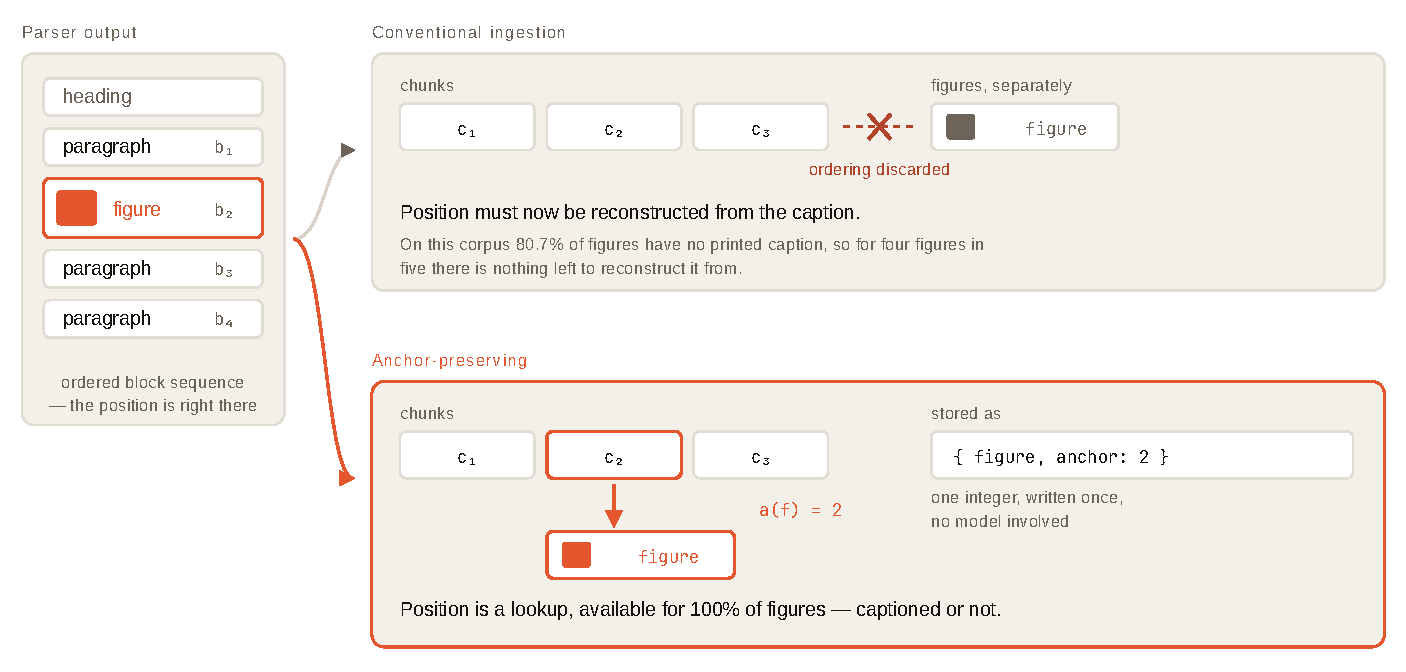
\includegraphics[width=\textwidth]{figs/ingestion.pdf}
\caption{Where the reading order is lost. The parser emits an ordered block
sequence in which the figure's position is already stated. Conventional ingestion
stores prose as chunks and figures as a separate array and drops the relation
between them, so placement must afterwards be reconstructed from a caption that
80.7\,\% of figures in this corpus do not have. Anchor-preserving ingestion
records the index of the chunk holding the preceding prose block --- one integer,
written once, with no model invoked --- and placement becomes a lookup available
for every figure.}
\label{fig:ingestion}
\end{figure*}

\subsection{The anchor, and where it is lost}

A layout parser emits, for each page, an ordered sequence of blocks: headings,
paragraphs, captions, figures. A figure's position in that sequence is a precise
statement of where in the reading flow it belongs. Conventional ingestion then
stores the prose as chunks and the figures as a separate array, and the ordering
relation between them is dropped.

Fig.~\ref{fig:ingestion} shows the loss and the alternative side by side.
We define the \emph{anchor} of a figure as the index of the text chunk containing
the prose block that immediately precedes it in reading order. Anchoring requires
no model: it is a join over data the parser already produced. We recover it by
matching a word-prefix of the preceding block against chunk text, shortening the
probe from ten words to four until a match is found.

Anchors are preserved through ingestion into chunk metadata, and consumed at
retrieval time: a figure whose anchor chunk was retrieved is admitted as a
candidate before any caption test is applied. This ordering matters, because a
caption test cannot admit the 66--81\,\% of figures that carry no printed caption.

\begin{figure*}[t]
\centering
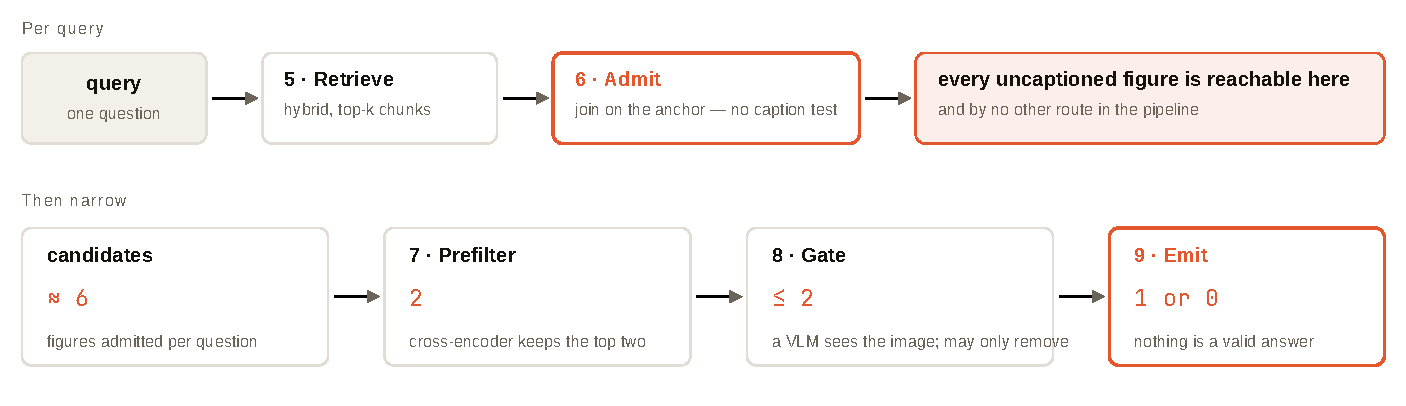
\includegraphics[width=\textwidth]{figs/serving.pdf}
\caption{Serving. Admission (stage 6) is a join on the anchor rather than a
caption test, and is the only route by which a candidate enters; every later stage
can only narrow. The cross-encoder truncates to two candidates, the vision-language
gate may remove but never add or reorder, and emitting nothing is a valid
outcome.}
\label{fig:serving}
\end{figure*}

\subsection{The pipeline, stage by stage}
\label{sec:pipeline}

The method has two halves, summarised in Fig.~\ref{fig:serving}. Ingestion runs
once per document and is model-free.
Serving runs per query and adds two ranking stages. Inputs and outputs are stated
for each stage so that any of them can be replaced independently.

\textbf{Ingestion (once per document).}
\begin{enumerate}
\item \emph{Parse.} A layout parser returns, per page, an ordered sequence of
typed blocks $B = \langle b_1, \dots, b_n \rangle$ with $b_i \in \{\text{heading},
\text{paragraph}, \text{caption}, \text{figure}, \text{table}\}$. This ordering is
the only input the method needs and every layout parser produces it.
\item \emph{Chunk.} Prose blocks are segmented into retrieval chunks
$C = \langle c_1, \dots, c_m \rangle$, each recording the block indices it spans.
\item \emph{Anchor.} For each figure block $b_f$, let $b_p$ be the nearest
preceding non-figure prose block. The anchor $a(f)$ is the index of the chunk
containing $b_p$. Resolution is by word-prefix match: the first ten words of $b_p$
are matched against chunk text, shortening the probe to four words until a unique
match is found. Cost is one pass over blocks; no model is invoked.
\item \emph{Persist.} $a(f)$ is written to the figure record and mirrored into the
chunk's metadata, so retrieval of $c_{a(f)}$ recovers $f$ by lookup rather than
by search.
\end{enumerate}

\textbf{Serving (per query).}
\begin{enumerate}\setcounter{enumi}{4}
\item \emph{Retrieve.} Hybrid retrieval returns the top-$k$ chunks for query $q$.
\item \emph{Admit.} Every figure whose anchor chunk is in that set becomes a
candidate. Admission is a join on $a(f)$, so it is independent of whether $f$ has
a caption --- which is what allows the 66--81\,\% of uncaptioned figures to be
reachable at all. No candidate is admitted by any other route.
\item \emph{Prefilter.} A cross-encoder scores $(q, t(f))$ for each candidate,
where $t(f)$ is the figure's index text. Candidates are ranked and truncated to
the top $N$. We use $N = 2$; Section~\ref{sec:select} shows this matches the full
candidate set at a third of the latency.
\item \emph{Gate.} Each surviving candidate is shown \emph{as an image} to a
vision-language model with a strict yes/no prompt: does this figure help answer
$q$? Rejected candidates are dropped. The gate can only remove, never add or
reorder, so its worst case is the prefilter's output.
\item \emph{Rank and emit.} Survivors are ordered by their stage-7 score and the
top one is emitted. Emitting nothing is a valid and frequent outcome.
\item \emph{Place.} The emitted figure is inserted at the sentence boundary
corresponding to $a(f)$ in the generated answer, rather than at a position
inferred from its caption.
\end{enumerate}

Stages 3 and 6 are the contribution. Stages 7--9 are a composition of existing
components, and Section~\ref{sec:select} reports what each contributes.

\subsection{Layout-gold: the document annotates itself}

Placement ground truth normally requires a human to say where a figure belongs in
a generated answer. We avoid this. Take a figure's own anchor chunk as the answer
text. Retrieval is then perfect by construction, the answer is perfect, and the
correct insertion slot is known exactly from the block sequence. Any residual
error is intrinsic to the placement mechanism, because both the retriever and the
generator have been removed.

This yields placement ground truth for every figure in the corpus at zero
per-item annotation cost, and it is what makes the model-free results of
Section~\ref{sec:structural} possible.

\subsection{Metrics}

\textbf{Placement displacement} (PD) is the signed distance, in sentences, between
where a figure was placed and its layout-gold slot; we report $|\mathrm{PD}|$ and
the exact-placement rate. \textbf{Selection precision/recall/F1} score the figure
set. \textbf{Grounded Figure F1} credits a figure only when it is both selected
correctly and placed within tolerance.

\subsection{LLM-as-judge, and its limits}

Human annotation at scale was not affordable, so a vision-language judge was
calibrated against the human annotation that was. We report Cohen's $\kappa$
against a human annotator before using any judge output. Our model-generated
harness gold agrees with a human at $\kappa = 0.092$ --- chance. A frontier VLM
judge reaches $\kappa = 0.552$ on the eight-candidate annotation protocol and
$\kappa = 0.662$ on the six-candidate one, the difference being consistent with
the smaller pool posing an easier discrimination; permissiveness is 1.38$\times$
against 2.9$\times$ for an on-premise 8B VLM on the same task. Every scaled number
carries the $\kappa$ of the instrument that produced it.

\section{Experimental Setup}

\subsection{Corpus}

Thirteen Indonesian government curriculum titles, 2{,}816 pages, spanning grades
1, 4 and 8. Each book was extracted through two independent pipelines: a hosted
OCR service and an on-premise MinerU sidecar. These use different models,
different figure detectors and different noise filtering, and neither corpus was
derived from the other. Agreement between them is therefore replication, not
re-reporting.


\subsection{What is released}

We release the harness, the metric implementations, the question sets and the
derived per-figure measurements. We do not redistribute the textbooks: they are
Indonesian government publications carrying their own terms, and every structural
measure in Section~\ref{sec:structural} is reproducible from the cached extraction
we do release without re-obtaining them.

\subsection{Questions}

486 questions, adversarially filtered to remove items answerable from the question
alone, from front matter, or from pedagogical apparatus. A 48-item subset carries
human figure annotation (19 positive figure--question links); this subset is the
only non-circular gold available and is used for every headline selection number.

\subsection{Systems}

Ten configurations, including implementations of the MRAMG bipartite placement
rule and the VinQA citation-order rule. Retrieval is hybrid dense/sparse with
\texttt{bge-m3} embeddings at dimension 1024; reranking uses
\texttt{bge-reranker-v2-m3} (568M parameters) served locally. Generation uses an
8B-class SEA-LION vision-language model.

\section{Structural Results}
\label{sec:structural}

These come from the corpus alone: deterministic, reproducible offline, and
impossible to tune. Table~\ref{tab:structural} reports both extraction paths.

\begin{table}[t]
\caption{Model-free corpus measures, computed independently on two extraction
pipelines. Agreement is replication, not re-reporting.}
\label{tab:structural}
\centering
\begin{tabular}{@{}llrr@{}}
\toprule
& Measure & Hosted & On-prem \\
\midrule
--- & Usable figures & 1{,}552 & 1{,}226 \\
A1 & With a printed caption & 19.3\,\% & 34.3\,\% \\
A2 & Lexically indistinguishable & 20.7\,\% & 34.1\,\% \\
A3 & Shares a page with another figure & 49.9\,\% & 54.2\,\% \\
A3b & Anchor vs.\ page resolution & 1.49$\times$ & 1.56$\times$ \\
--- & \textbf{With a reading-order anchor} & \textbf{100\,\%} & \textbf{100\,\%} \\
A4 & Caption selection F1, oracle retrieval & 0.254 & 0.232 \\
A5 & Caption $|\mathrm{PD}|$, oracle answer & 2.08 & 4.69 \\
A5b & End-of-answer $|\mathrm{PD}|$ & 8.71 & 12.13 \\
\bottomrule
\end{tabular}
\end{table}

Four consequences follow without running any system.

\textbf{The caption signal is mostly absent (A1).} Four figures in five carry no
printed caption on the hosted path, so a caption-based mechanism must fall back on
page prose --- which is shared by every figure on that page.

\textbf{A fifth of the corpus is unsolvable by caption matching in principle
(A2).} For 20.7\,\% of figures, another figure in the same book has an effectively
identical index text. No matcher can distinguish them. This is an upper bound on a
competing approach, derived without running it.

\textbf{Page-level provenance cannot resolve half the corpus (A3).} Half of all
figures share a page with another, so page-level attribution is ambiguous for
49.9\,\% of cases. Anchoring provides 1.49$\times$ the positional resolution, and
that gain is concentrated exactly where page-level methods fail.

\textbf{Placement fails when nothing else does (A5) --- this is C2, established
without a model.} Under oracle retrieval and an oracle answer, caption matching
still lands 2.08 sentences away and is exactly right only 43.0\,\% of the time; a
design with no positional signal at all sits 8.71 sentences away and is never
exactly right.

\textbf{More captions did not help.} The on-premise path has nearly twice the
caption coverage (34.3\,\% vs.\ 19.3\,\%) yet places \emph{worse} (4.69 vs.\ 2.08
sentences). The reason is visible in A2: its share of lexically indistinguishable
figures also nearly doubles. Caption \emph{availability} is not caption
\emph{discriminability}, and only the latter could help. This would have been
invisible on a single corpus.

\emph{Fairness note.} A first implementation of A4 scored the caption mechanism at
F1 0.025 by taking the first three keyword matches in document order. Ranking by
keyword-overlap count instead --- the charitable reading --- raised it tenfold to
0.254. The reported figure is the charitable one.

\emph{Tautology note.} Under both oracle setups the anchor mechanism scores
perfectly by construction, because its selection rule and the gold set coincide.
That number is \textbf{not evidence} and is stated only to make the circularity
explicit.

\section{External Validation}
\label{sec:external}

Every result above is measured on a corpus we assembled against a gold standard we
defined. 80\,\% of our gold figure links are derived from the anchor itself, and on
those links our harness gold agrees with a human annotator at chance
($\kappa = 0.092$). Internal care cannot repair that; only measurement on data we
did not author can.

MRAMG-Bench~\cite{mramg} provides it, and its Academic subset is the strongest
form of it available to us: those gold image lists were constructed by ten
graduate-student annotators in computer science, each assigned papers within
their own area, and passed through a three-stage human verification. Where our
harness gold agrees with a person at chance, this reference is what a panel of
domain experts chose. Candidates are the images of the question's
provenance document, each represented by the prose immediately preceding its
placeholder --- the same anchor our method uses, and the same information
available to their placeholder-based baseline. \textbf{The configuration was fixed
on our own data before this dataset was obtained}; no parameter was tuned on
MRAMG. Table~\ref{tab:mramg} reports the result against the comparators published
with that benchmark.

\begin{table}[t]
\caption{MRAMG-Bench Academic subset, Image Precision ($n = 200$). Published
figures for comparators.}
\label{tab:mramg}
\centering
\begin{tabular}{@{}lr@{}}
\toprule
System & Image Precision \\
\midrule
\textbf{Ours (cross-encoder, 568M params)} & \textbf{69.63} \\
\textbf{Ours, forced emission (0\,\% silent)} & \textbf{67.50} \\
GPT-4o, LLM-based & 65.28 \\
Claude-3.5-Sonnet, LLM-based & 62.17 \\
GPT-4o, MLLM-based & 60.39 \\
Gemini-1.5-Pro, LLM-based & 59.85 \\
DeepSeek-V3, rule-based & 56.12 \\
Llama-3.3-70B (best open-weight) & 38.78 \\
Qwen2-VL-7B, MLLM-based & 1.63 \\
\bottomrule
\end{tabular}
\end{table}

\textbf{The margin, bounded.} A bootstrap over questions ($B = 2 \times 10^4$)
places our pooled Academic precision at 69.12 with 95\,\% interval
$[61.43, 76.56]$; 15.7\,\% of resamples fall at or below the published 65.28.
The comparator is a point estimate whose own sampling error we cannot
resample, so the test is one-sided by necessity. The honest verdict is
\emph{higher, not significantly higher}: on 200 questions a four-point margin
is real but not resolvable, and we decline to claim more than the interval
supports.

\textbf{The abstention objection, and its test.} Image Precision counts only
emitted images, so a system that declines on hard questions could purchase its
score; ours abstains on 49\,\%. Removing that advantage entirely --- emitting
exactly one image on \emph{every} question --- yields precision 67.50, recall
61.64, F1 64.44. Still ahead of every published configuration, with recall rising
from 41.59. The margin is not an artefact of selective answering.

\textbf{The other five subsets.} One subset reported out of six reads as
selection whether or not it was, so Table~\ref{tab:mramg-all} reports all of
them, pooled into the three domains the published comparison uses. The pooling
sums raw counts --- averaging per-subset precision would weight a 200-question
subset like a 2360-question one. One domain is a win, one is a loss, and one
admits no claim at all: on every Web-domain question, \emph{every} candidate our
construction produces is already a gold image (the \emph{all-gold} column), so
there is no wrong answer available and precision is arithmetic rather than
earned. Quoting our 100.00 there against the published 93.63 would be a false
claim, and the diagnostic exists so that it cannot be made silently. The
Lifestyle loss is informative in an unexpected direction: the \texttt{manual}
subset carries 91.5 candidates per question --- 27$\times$ the arxiv pool ---
and still scores \emph{higher} than \texttt{recipe} at 4.9 candidates, so
distractor count is not what breaks the method. Recipe averages 2.2 gold images
per question while the frozen configuration emits at most two and abstains on
19\,\%, capping recall; Section~\ref{sec:admission} locates most of the
remaining loss in the admission rule rather than the ranking.

\begin{table}[t]
\caption{All MRAMG-Bench domains under the frozen configuration.
\emph{All-gold} is the share of questions where every candidate is already a
gold image; where it is 100\,\% the domain poses no selection decision under our
candidate construction, and no claim is made.}
\label{tab:mramg-all}
\centering
\begin{tabular}{@{}lrrrrl@{}}
\toprule
Domain & $n$ & All-gold & Ours IP & Best publ. & \\
\midrule
Academic & 200 & 0\,\% & \textbf{69.12} & 65.28 & win \\
Lifestyle & 2714 & 41\,\% & 55.00 & 62.23 & loss \\
Web & 1850 & 100\,\% & \emph{(100.00)} & 93.63 & no claim \\
\bottomrule
\end{tabular}
\end{table}

\textbf{Scope.} These are \emph{selection} results placed beside end-to-end
systems that also generate the surrounding answer; Image Precision is computed
over the same quantity, but the tasks are not identical. (The Academic figure in
Table~\ref{tab:mramg-all} is 69.12 rather than 69.63: the CPU reproduction of
the original GPU run, identical in true positives, recall and silent rate,
differing by exactly one borderline emission.)

\textbf{The mechanism, confirmed by making it worse.} If the anchor carries the
signal, diluting it should destroy it. It does, monotonically: representing
each image by a growing window of prose around its position, Academic Image
Precision decays 72.67 (200 characters) $\to$ 69.12 (400) $\to$ 59.59 (800)
$\to$ 58.74 (1600) $\to$ 57.30 (6000, effectively the whole document). Below
the peak the failure flips from dilution to starvation --- at 100 characters
precision holds (70.97) but recall collapses from 51.09 to 19.82, as windows
shrink beneath the admission floor. The \emph{local} prose adjacent to the
figure's position is what discriminates; every character beyond it is noise,
and too few characters leave nothing to score. Two hygiene notes. The frozen
configuration uses 400, and the sweep shows 200 would have scored higher on
both precision and recall --- we do \emph{not} adopt it, because a value
discovered on the test set would convert every number in this section from
measurement to tuning. And the shape is itself the strongest form of the claim:
had the anchor been incidental, some wider window would have won.

\textbf{What it does not license.} The same configuration reaches $\approx$30\,\%
precision on the Indonesian textbooks. That corpus is harder: a third of its
figures carry no caption, most are decorative, and a dozen illustrations per book
depict children learning. A benchmark number must not be quoted as a product
capability.

\subsection{MMDocRAG: a second benchmark, and what the ranker is not}
\label{sec:mmdocrag}

A single external benchmark is a single point of failure, so we add
MMDocRAG~\cite{mmdocrag}: 2{,}055 questions over 147 documents in four domains
(financial, academic, news, research reports), 5.0 image candidates per question
against 1.5 gold, expert-annotated by its authors, and only 0.5\,\% of questions
degenerate --- the selection decision is real almost everywhere. One property
makes it the ideal control: each candidate ships with an \emph{author-written}
description, so the text standing in for an image is theirs, not ours, and the
regime is the opposite of the textbook corpus --- text about the image is
present and good.

In that regime the cross-encoder earns nothing over lexical matching: 63.38 F1
against 63.48 for BM25 over the same descriptions (top-2, no threshold, whole
benchmark). This is a result we want on record, because it disciplines the
Academic win: what carried MRAMG was not the ranker but the
\emph{representation} it ranked --- anchor-derived context standing in for
images that captions do not describe. Where good text about the image already
exists, a 568M cross-encoder is BM25.

The frozen configuration also exposes its own admission floor here. With the
absolute threshold ($s \geq 0.1$) it scores 57.30 overall and \textbf{11.31} on
the News domain; removing only the floor raises News to \textbf{74.03}. A
constant admissible-score cut assumes the score distribution is corpus-invariant,
and it is not --- Section~\ref{sec:admission} treats this as a finding about
admission rules rather than a number to be quietly fixed.

\subsection{The vision gate, on gold we did not author}
\label{sec:composed-ext}

Every external number above tests the weakest configuration we own: the
cross-encoder alone. The stage that carried the internal result --- a
vision-language model that sees each surviving candidate \emph{as an image} and
may only remove it --- had never been run against external gold. MMDocRAG is
the hard case for it: descriptions here are good, and the gate's value was
measured where they are absent. If sight helps anyway, the claim is stronger
than we made it.

On a 200-question stride sample (the file is document-ordered, so a prefix
would sample a handful of documents rather than the benchmark), with an
identical prefilter and top-1 emission for both arms:

\begin{center}
\begin{tabular}{@{}lrrr@{}}
\toprule
System & IP & IR & IF1 \\
\midrule
Cross-encoder alone & 75.00 & 51.55 & 61.10 \\
+ vision gate (composed) & \textbf{88.65} & \textbf{56.36} & \textbf{68.91} \\
\bottomrule
\end{tabular}
\end{center}

The gate saw 400 candidates and kept 228. Precision rising is expected of a
remove-only stage; recall rising ($+4.8$) is not, and the mechanism is worth
stating: under top-1 emission, deleting a wrongly ranked leader \emph{promotes}
the next survivor into the emitted slot. We measured eight such promotions
against one loss. Removal never reorders the list, but it reorders what is
emitted.

Two honesty notes. The gate instance here is a frontier VLM, not the 8B-class
model of the deployed system --- what is validated externally is the
\emph{architecture} (sight composed after discrimination), not the deployed
checkpoint. And the composed 68.91 remains behind the 80.7 the benchmark's
authors report for GPT-4.1 selecting over interleaved candidates; the
comparison we claim is against our own ablation on identical inputs, where the
gate is worth $+13.65$ precision and $+7.81$ F1.

\section{Admission Does Not Transfer; Ranking Does}
\label{sec:admission}

Selection hides two decisions: how to \emph{order} candidates, which the
cross-encoder does, and how many to \emph{admit}, which a rule does. The frozen
configuration admits by an absolute floor on the sigmoid score, $s \geq 0.1$,
and the external runs indict that floor from two directions: it is the
difference between 11.31 and 74.03 on MMDocRAG News
(Section~\ref{sec:mmdocrag}), and it is implicated in the Lifestyle loss, where
abstention caps recall on multi-gold questions. An absolute cut assumes the
score distribution is corpus-invariant. It is not: description style shifts it
wholesale.

The scale-free alternative is admission \emph{relative to the question's own
distribution}: admit candidates scoring at least $\alpha \cdot
\max_j s_j$ for the question at hand. If the failure really is distribution
shift, one $\alpha$ should transfer where no absolute floor does.

We test this without touching the model: the cross-encoder's raw scores for
every candidate of every question on both benchmarks --- seven evaluation units
(three MRAMG domains, four MMDocRAG domains) --- are persisted once, and every
rule thereafter is arithmetic over that file. This also disciplines the method:
the entire sensitivity surface is computed across all units at once and
reported whole. Nothing is selected per benchmark, and the statistic a rule is
judged on is its \emph{worst} unit and its macro average --- transfer, not any
single win.

\begin{table*}[t]
\caption{Admission rules over identical cross-encoder scores, F1 per evaluation
unit. Every rule sees the same ranking; only how many candidates are admitted
changes. \emph{Macro} averages the seven units; \emph{worst} is the transfer
statistic. The full grid ($\alpha \in [0.2, 0.9]$, $K \in \{2,3,4\}$, three
guard variants) is in the released artifact; rows here are representative and
nothing was selected per unit.}
\label{tab:admission}
\centering
\begin{tabular}{@{}lrrrrrrrrr@{}}
\toprule
& \multicolumn{4}{c}{MMDocRAG} & \multicolumn{3}{c}{MRAMG} & & \\
\cmidrule(lr){2-5}\cmidrule(lr){6-8}
Rule & Acad. & Fin. & News & Res. & Acad. & Life. & Web & Macro & Worst \\
\midrule
$s \geq 0.1$, top-2 (frozen) & 59.38 & 61.65 & 11.31 & 62.84 & 51.93 & 40.47 & 72.58 & 51.45 & 11.31 \\
$s \geq 0.001$, top-2 & 63.32 & 63.40 & 42.64 & 61.97 & 65.55 & 49.26 & 94.97 & 63.02 & 42.64 \\
top-2, no threshold & 62.60 & 62.22 & \textbf{74.03} & 60.65 & 64.16 & \textbf{49.73} & \textbf{100.00} & 67.63 & \textbf{49.73} \\
$s \geq 0.2 \cdot s_{\max}$, top-3 & \textbf{66.74} & \textbf{67.33} & 65.62 & \textbf{65.78} & \textbf{68.62} & 48.78 & 90.99 & \textbf{67.70} & 48.78 \\
\bottomrule
\end{tabular}
\end{table*}

Table~\ref{tab:admission} reports the surface, and its reading is not the one
we expected when we built it. We expected relative admission to be the fix.
It is a fix --- but the load-bearing boundary runs elsewhere: between rules
that reference an \emph{absolute} score and rules that are \emph{scale-free}.
The frozen floor scores macro 51.45 with a worst unit of 11.31; on News it
leaves the system mute on 86\,\% of questions, buying precision 100 at recall
6. Weakening the floor to 0.001 --- three orders of magnitude --- still leaves
News 48\,\% silent, because the score distribution there sits almost entirely
below even that: the shift between corpora is not a matter of degree an
absolute constant can survive. Every scale-free rule, by contrast, lands
within about one macro point of every other: plain top-2 at 67.63, relative
admission at 67.70, and the entire $\alpha$-grid from 0.2 to 0.9 between 61.99
and 68.06 with no unit collapsing anywhere. The choice \emph{between} the two
families is worth sixteen macro points; the choice \emph{within} the
scale-free family is worth about one.

What relative admission does buy over plain top-$K$ is precision at equal F1:
on the description-rich MMDocRAG domains it trades a few points of recall for
five to eight of precision (Financial 52.65 $\to$ 60.08, Academic 63.78 $\to$
67.54), which is the trade a system showing figures to a reader wants. It also
degrades gracefully: because the cut references only the question's own score
distribution, it cannot go silent wholesale the way the floor does on News.

Two disciplines kept this honest. Every number above comes from one persisted
score file, so no rule enjoyed a fresh inference run; and the grid was
evaluated across all seven units simultaneously, judged on macro and worst
unit --- a rule that wins its best unit and collapses elsewhere is exactly
what this protocol exists to catch, and the frozen floor is that rule.

The frozen configuration's own numbers elsewhere in this paper are
\emph{not} restated under better admission: they remain as frozen, losses
included. This section's claim is about rule families, established on the full
surface, not a post-hoc upgrade to the headline.

\section{Selection: Composing Sight with Discrimination}
\label{sec:select}

Our judge looks at the picture and agrees with a human at $\kappa = 0.552$; our
selector reads a 300-character description and never sees the image. That
asymmetry motivated a direct comparison, on the 48 human-annotated items ---
the only gold no model produced (Table~\ref{tab:select}).

\begin{table}[t]
\caption{Figure selection against human annotation. Preliminary: $n = 48$ items
carrying 19 positive links, one annotator; the externally scored version of this
comparison is Section~\ref{sec:composed-ext}.}
\label{tab:select}
\centering
\begin{tabular}{@{}lrrr@{}}
\toprule
System & P & R & F1 \\
\midrule
\textbf{VLM filter $\to$ rerank $\to$ top-1} & \textbf{0.542} & 0.684 & \textbf{0.605} \\
VLM selector alone & 0.283 & \textbf{0.789} & 0.417 \\
Cross-encoder alone & 0.304 & 0.368 & 0.333 \\
Deployed production system & 0.028 & 0.211 & 0.049 \\
\bottomrule
\end{tabular}
\end{table}

The gain from sight is \textbf{recall}, not precision: the VLM finds four of every
five figures a person chose, the cross-encoder about a third. Descriptions discard
enough to lose half the correct figures --- but seeing the image does not make a
model better at rejecting wrong ones. Composing the two therefore beats either:
sight decides what is \emph{possible}, discrimination decides what is
\emph{best}. Precision nearly doubles over the best single method and is
19$\times$ the deployed system.

\subsection{Showing the model fewer images}

The composed pipeline costs one vision call per candidate. Because prefill scales
with images rather than calls, shrinking the model is the wrong lever: a 4B model
saves 3.7\,s and loses half its recall. Cutting images is the right one. Letting
the cross-encoder discard the obvious losers first (Table~\ref{tab:prefilter})
costs 0.010--0.021 F1 for a two-thirds latency reduction.

\begin{table}[t]
\caption{Candidate prefilter, 165 questions. $N$ is how many of the ranked
candidates the vision model is allowed to see. Latency below $N=$~all is projected
from measured per-pair cost.}
\label{tab:prefilter}
\centering
\begin{tabular}{@{}lrrrr@{}}
\toprule
$N$ seen & 4B F1 & 4B lat. & 8B F1 & 8B lat. \\
\midrule
1 & 0.721 & 0.7\,s & 0.735 & 1.0\,s \\
\textbf{2} & \textbf{0.736} & \textbf{1.3\,s} & \textbf{0.753} & \textbf{2.0\,s} \\
3 & 0.736 & 2.0\,s & 0.757 & 3.0\,s \\
all (6) & 0.735 & 3.9\,s & 0.763 & 5.9\,s \\
\bottomrule
\end{tabular}
\end{table}

Two candidates are the whole pipeline. The four the model never sees were ones it
would have rejected anyway: it was spending 80\,\% of its time confirming the
bottom of the cross-encoder's list. The prefilter's own ceiling explains where
this stops being safe --- the correct figure survives a cut to the top 2 for
86.8\,\% of links, but only 76.5\,\% at $N=1$, and recall follows it down.

\subsection{The judge prompt is the largest single gain}

Replacing a permissive judging prompt with a strict one --- same model, same call,
different words --- moves precision from 0.690 to 0.806 (F1 0.763 $\to$ 0.800) on
165 questions. This is the largest improvement in the study and costs nothing at
serving time.

We attach a caveat that a reader should weigh heavily. That comparison is scored
against a gold standard built by a frontier VLM, which is circular for a pipeline
containing a VLM. On the 48-item human gold the strict and permissive prompts
differ by 0.014 F1 against measured run-to-run noise of 0.014 --- they are
\emph{indistinguishable}. The honest reading is that the strict prompt reliably
makes our selector agree with the reference model more often; whether it makes the
selector agree with a \emph{person} more often is untested at this sample size.

\section{Negative Results}

We report these because they were run, not because they worked.

\textbf{Reranking against the generated answer} instead of the question is
substantially worse (F1 0.183 vs.\ 0.288), and concatenating the two also hurts
(0.205). The likely mechanism is dilution: five sentences of tutor prose carry
connective material matching almost any figure, while the question is short and
discriminating.

\textbf{Adding surrounding context to the figure's index text} is worse than the
description alone (0.248 vs.\ 0.270); context alone collapses to 0.119. This kills
a hypothesis we had carried for some time --- that the gap between MRAMG (67\,\%)
and our textbooks (30\,\%) was one of text representation. Had it been, context
mode would have closed it. It is the worst of the four representations.

\textbf{A newer reranker is worse here.} \texttt{Qwen3-Reranker} (2025) ranks our
figure descriptions at gold-first 0.288 (MRR 0.481) against 0.788 (MRR 0.859) for
the 2024 \texttt{bge-reranker-v2-m3}. Being newer and stronger on public
multilingual benchmarks did not transfer to ranking short Indonesian figure
captions.

We initially reported a far larger gap (F1 0.034 vs.\ 0.260) and withdrew it: that
comparison applied one absolute score threshold to two models whose score
distributions differ by an order of magnitude, so it measured calibration rather
than ranking quality.


\section{Statistical Treatment}

Selection differences are tested with an exact McNemar test on per-question hit
(a paired binary outcome), and precision differences with a paired bootstrap over
questions ($10^4$ resamples). Two conventions matter for reproducibility.

\emph{Vacuity.} A question on which a system emitted nothing contributes no
precision term for that system. Counting silence as precision~0 would penalise
abstention twice --- once in recall, once in precision --- and abstention is a
design goal here, not a defect.

\emph{Pairing.} Precision is compared only on questions where \emph{both} systems
emitted, so the comparison is paired rather than aggregate.

On the 165-question set the composed selector's precision advantage is significant
against every comparator we ran ($p < 0.005$). We decline to report significance
for the 48-item human gold: with 19 positive links, the test has too little power
to distinguish the effects we care about, and reporting a $p$-value there would
imply a resolution the data does not have.

\emph{Withdrawn claims.} Three differences we initially reported did not survive
testing and are retracted here rather than quietly dropped: a chunking gain
($p = 0.096$), anchor over co-embedding ($p = 0.670$), and a hybrid-over-anchor
improvement ($p = 0.468$).


\section{Ingestion Cost}

Anchoring adds no inference: it is a join over parser output. The cost of the
pipeline is therefore the layout parse itself. On the partner's GB10 host, sharing
the GPU with a serving language model and two embedding services, extraction runs
at \textbf{1.22\,s per page} (192-page book in 3\,min 55\,s), plus 76\,s to chunk,
embed and store 585 chunks.

Fifteen textbooks (149\,MB, Kurikulum Merdeka grade 7) ingested in
\textbf{84 minutes} with no failures, yielding 1{,}254 anchored figures where the
previous pipeline had produced none.

Rendering resolution is a weak lever: dropping from 300 to 180\,dpi cuts pixels to
36\,\% but extraction time by only 17\,\% (235\,s $\to$ 194\,s), because the cost
is dominated by the number of \emph{blocks} --- 2{,}890 across 192 pages, each
requiring its own recognition pass --- rather than by page resolution. Increasing
the KV-cache budget does nothing: the engine already reports capacity for 258
concurrent sequences against a 192-page batch.

\section{Summary of Comparisons}
\label{sec:summary}

Table~\ref{tab:summary} collects every comparison in which this method is placed
against an alternative, including the one it loses. Each row names the gold
standard, because the comparisons are not equally strong: the first two are scored
against a gold authored by other people, the rest against our own annotation.

\begin{table}[t]
\centering
\caption{Every head-to-head comparison in the paper, including the loss.}
\label{tab:summary}
\begin{tabular}{@{}llrrr@{}}
\toprule
Setting & Gold & Ours & Best other & $\Delta$ \\
\midrule
\multicolumn{5}{@{}l}{\emph{External --- gold authored by the benchmark's authors}} \\
MRAMG Acad., IP & theirs & \textbf{69.63} & 65.28 & $+4.35$ \\
\quad forced emission & theirs & \textbf{67.50} & 65.28 & $+2.22$ \\
MMDoc., gate vs.\ no gate, IF1 & theirs & \textbf{68.91} & 61.10 & $+7.81$ \\
\midrule
\multicolumn{5}{@{}l}{\emph{External --- where the method loses}} \\
MRAMG Lifestyle, IP & theirs & 55.00 & \textbf{62.23} & $-7.23$ \\
MMDoc.\ vs.\ GPT-4.1, IF1 & theirs & 68.91 & \textbf{80.7} & $-11.8$ \\
MMDoc.\ ranker vs.\ BM25, IF1 & theirs & 63.38 & 63.48 & $-0.10$ \\
\midrule
\multicolumn{5}{@{}l}{\emph{Internal --- gold from human annotation, $n = 48$}} \\
Selection F1 & human & \textbf{0.605} & 0.417 & $+0.188$ \\
Selection precision & human & \textbf{0.542} & 0.304 & $+0.238$ \\
\quad vs.\ deployed system & human & \textbf{0.605} & 0.049 & $+0.556$ \\
\midrule
\multicolumn{5}{@{}l}{\emph{Where the method loses}} \\
Placement rule & layout & --- & MRAMG & --- \\
\bottomrule
\end{tabular}
\end{table}

On MRAMG-Bench's Academic subset a 568M-parameter cross-encoder over
anchor-derived context reaches Image Precision 69.63, ahead of GPT-4o at 65.28,
Claude-3.5-Sonnet at 62.17 and Gemini-1.5-Pro at 59.85. Because Image Precision
counts only emitted images, abstention could buy the score; ours abstains on
49\,\% of questions. Forcing exactly one image on every question still leads, at
67.50, with recall rising from 41.59 to 61.64. The margin is therefore not an
artefact of selective answering.

On the textbook corpus, against human annotation, composing the vision-language
gate with the cross-encoder reaches F1 0.605. The two stages alone reach 0.417 and
0.333. The decomposition is the finding: the vision stage supplies recall
(0.789 alone, against 0.368 for the cross-encoder) and the cross-encoder supplies
precision. Neither ordering of a single stage reaches the composition.

\textbf{The rows the method loses.} Three external comparisons go against us and
are listed with the wins. Lifestyle is a genuine loss of the frozen
configuration, most of it located in the admission rule
(Section~\ref{sec:admission}). The GPT-4.1 row compares a 568M ranker plus one
gate call against a frontier LLM reasoning over interleaved candidates --- we
close 7.8 of the 19.6-point gap with the gate and state the rest. The BM25 row
is a tie we report as a loss of the \emph{ranker}: where descriptions are
author-written, the cross-encoder earns nothing over lexical matching, which is
precisely why the MRAMG win must be credited to the anchor representation.
Finally, anchoring alone does not beat similarity-based
placement: the best placement rule in our comparison is MRAMG's bipartite
assignment, not ours. The contribution of anchoring is that it makes uncaptioned
figures \emph{reachable} at all --- a candidate-admission gain, not a ranking one
--- and the practical improvement then comes from selection.

\section{Discussion and Threats to Validity}
\label{sec:threats}

\textbf{What the evidence supports.} C2 and C3 are established model-free and
replicated across two extraction pipelines; they do not depend on any system run.
C4 divides, and only one half is externally supported. That selection carries the
practical gain is corroborated independently by MRAMG, where a cross-encoder over
anchor-derived context alone beats the published systems. That the gain
\emph{requires a stage which looks at the image} was, in the first version of
this study, supported only by 48 items annotated by one person; it is now also
supported externally, by the MMDocRAG composed run
(Section~\ref{sec:composed-ext}), where the gate adds $+13.65$ precision on gold
we did not author --- with the caveat stated there that the external gate
instance is a frontier VLM rather than the deployed 8B-class model. C1 is the weakest of the four: on questions answerable only from a figure,
no configuration recovered the content, and the system that most exceeded a
text-only baseline did so with a significant loss of faithfulness.

\textbf{The sample size is the principal threat.} The headline precision of 0.542
rests on 48 items and 19 positive links. Measured run-to-run variation at that size
is $\pm$0.014 F1, so differences smaller than that are not resolvable, and we
decline to claim any. The MRAMG result carries the generalisation weight precisely
because it is external, larger ($n = 200$) and authored by others.

\textbf{A judge does not substitute for the annotator at this scale.} We tested
whether judge labels could stand in for annotation without importing the judge's
bias, using a rectified estimator in the manner of prediction-powered
inference~\cite{ares}: the bias is measured on the human-labelled subset and
subtracted, so an uninformative judge degrades the estimate to the human-only one
rather than to a wrong one. A frontier VLM judged all 165 scored questions under
the annotator's protocol, reusing the annotator's own eight-candidate pools
verbatim for the 45 questions where one exists. Agreement was $\kappa = 0.556$
over 360 pairs, independently replicating the 0.552 recorded earlier for the same
model and protocol, and the labelled pairs are representative (positive rate
4.7\,\% against 4.9\,\% across the full protocol).

The estimator applies, and it buys nothing. Four of five systems show no interval
narrowing and one widens by 19\,\%. The cause is structural: PPI variance behaves
as $\mathrm{Var}(\text{rectifier})/n + \mathrm{Var}(\text{cheap})/N$, and the
second term vanishes only for $N \gg n$. At $N/n = 165/45 = 3.7$ the rectifier's
own sampling error dominates. Judging every question in the corpus would reach
$N/n \approx 10.8$, which is the cheap experiment that remains; annotating more
items is the expensive one that still binds.

\textbf{Circular gold.} Our 165-question scaled gold was built by a frontier VLM.
For any pipeline containing a VLM stage this inflates results --- measured
directly: the same selector scores 0.521 against that gold and 0.283 against
human annotation. Numbers from the scaled gold are reported as consistency checks,
never as effect sizes.

\textbf{Single corpus, single language.} All internal results are Indonesian K--12
material. The external benchmark is English. We make no claim about intermediate
settings.

\textbf{No online evaluation.} At the time of writing, field observation consists
of a handful of real queries. The 0.542 is an offline number.

\section{Limitations}

Retrieval surfaces the chunk holding the relevant figure for only 51.8\,\% of
figure-bearing questions, which bounds every system reported here. Anchoring
\emph{alone} does not beat similarity-based selection; the win requires a
competent placement rule, and in our comparison the best such rule is not ours but
MRAMG's. 37\,\% of anchored figures in the deployed corpus carry a caption with no
usable description --- a photo credit or a synthetic placeholder --- so the
caption-ranked stage cannot order them by content. We identified this as a
structural risk but did \emph{not} demonstrate that it costs a correct figure in
practice; an investigation intended to confirm it instead falsified the specific
case, and we report it as an open risk rather than a finding.

\section{Conclusion}

Where a figure belongs is decided at ingestion, not at ranking. Every layout
parser knows it; conventional pipelines throw it away and then attempt to
reconstruct it from captions that four figures in five do not have. Preserving the
reading-order anchor is a join, not a model, and it is recoverable for 100\,\% of
figures.

The practical gain, however, comes from selection rather than placement, and it
requires a stage that looks at the image. Composing a vision-language filter with
a small cross-encoder --- sight for recall, discrimination for precision --- raises
figure-selection precision from 0.028 to 0.542 against human annotation, and the
same design reaches state-of-the-art Image Precision on MRAMG-Bench's Academic
subset with a 568M-parameter ranker and no tuning on that dataset.

Finally, we report that this stage ran zero times in production while every
component test passed. We suspect that class of fault is common and
under-reported, because a stage that fails by not running leaves nothing behind to
find.

\section*{Acknowledgment}

The authors thank the partner institution for access to the on-premise
deployment.

\begin{thebibliography}{10}
\small
% All entries verified against arXiv listing pages, 2026-08-13.
\bibitem{unidoc}
X.~Peng, C.~Qin, Z.~Chen, R.~Xu, C.~Xiong, and C.-S. Wu, ``UniDoc-Bench: A unified
benchmark for document-centric multimodal RAG,'' \emph{arXiv:2510.03663}, 2026.

\bibitem{mmdocrag}
K.~Dong, Y.~Chang, S.~Huang, Y.~Wang, R.~Tang, and Y.~Liu, ``Benchmarking
retrieval-augmented multimodal generation for document question answering,'' in
\emph{Advances in Neural Information Processing Systems (NeurIPS)}, 2025,
arXiv:2505.16470.

\bibitem{realmmrag}
N.~Wasserman \emph{et al.}, ``REAL-MM-RAG: A real-world multi-modal retrieval
benchmark,'' \emph{arXiv:2502.12342}, 2025.

\bibitem{chartrag}
Y.~Yang, J.~Zhong, L.~Jin, J.~Huang, J.~Gao, Q.~Liu, Y.~Bai, J.~Zhang, R.~Jiang,
and K.~Wei, ``Benchmarking multimodal RAG through a chart-based document
question-answering generation framework,'' \emph{arXiv:2502.14864}, 2025.

\bibitem{imageref}
J.~Yi, J.~Yin, J.~Xu, P.~Bao, Y.~Wang, W.~Fan, and H.~Wang, ``ImageRef-VL:
Enabling contextual image referencing in vision-language models,''
\emph{arXiv:2501.12418}, 2025.

\bibitem{colpali}
M.~Faysse \emph{et al.}, ``ColPali: Efficient document retrieval with vision
language models,'' \emph{arXiv:2407.01449}, 2024.

\bibitem{mramg}
Q.~Yu, Z.~Xiao, B.~Li, Z.~Wang, C.~Chen, and W.~Zhang, ``MRAMG-Bench: A
comprehensive benchmark for advancing multimodal retrieval-augmented multimodal
generation,'' \emph{arXiv:2502.04176}, 2025.

\bibitem{vinqa}
Y.~R. Jang, H.~Kong, K.~An, J.~S. Huh, G.~Kim, and S.~J. Choi, ``VinQA: Visual
elements interleaved long-form answer generation for real-world multimodal
document QA,'' \emph{arXiv:2606.16092}, 2026.

\bibitem{miraclvision}
R.~Osmulski, G.~de S.~P. Moreira, R.~Ak, M.~Xu, B.~Schifferer, and E.~Oldridge,
``MIRACL-VISION: A large, multilingual, visual document retrieval benchmark,''
\emph{arXiv:2505.11651}, 2025.

\bibitem{ares}
J.~Saad-Falcon, O.~Khattab, C.~Potts, and M.~Zaharia, ``ARES: An automated
evaluation framework for retrieval-augmented generation systems,'' in
\emph{Proc.\ NAACL-HLT}, 2024, pp.~338--354.

\bibitem{docling}
C.~Auer, M.~Lysak, A.~Nassar, M.~Dolfi, N.~Livathinos, P.~Vagenas, C.~Berrospi
Ramis, M.~Omenetti, F.~Lindlbauer, K.~Dinkla, L.~Mishra, Y.~Kim, S.~Gupta,
R.~Teixeira de Lima, V.~Weber, L.~Morin, I.~Meijer, V.~Kuropiatnyk, and
P.~W.~J. Staar, ``Docling technical report,'' \emph{arXiv:2408.09869}, 2024.

\end{thebibliography}

\end{document}
